\documentclass[a4paper]{article}
\usepackage[title]{appendix}
\usepackage{authblk}
\usepackage{mathptmx}
\usepackage{url,latexsym,amsmath,amsthm,xspace,rotating,multirow,multicol,xspace,amssymb,paralist}
\usepackage{euscript}
\usepackage{fancybox,xcolor}
\usepackage{longtable}
\usepackage{paralist}
\usepackage[normalem]{ulem}
\usepackage[pdftex]{hyperref}
\usepackage{algorithmicx}
\usepackage{algpseudocode}
\usepackage{algorithm}
\usepackage{cancel}
\usepackage{mathtools}
\usepackage{fullpage}
\usepackage[nodayofweek]{datetime}

\usepackage{url}
\usepackage{latexsym}

\usepackage{times}
\usepackage{amsmath}
\usepackage{amsthm}
\usepackage{amssymb}
\usepackage{graphicx}
\usepackage{xspace}
\usepackage{tabularx}
\usepackage{multicol}
\usepackage{multirow}
%\usepackage{hyperref}
\usepackage{url}
%\usepackage{natbib}
\usepackage{wrapfig}
\usepackage{comment}
\usepackage{listings}
\usepackage{color}
\usepackage[utf8]{inputenc}
\usepackage{fancyvrb}
\usepackage{booktabs}
\usepackage{color}
\usepackage[normalem]{ulem}

\usepackage{textcomp}

\newcommand{\obs}{\text{obs}}
\newcommand{\mis}{\text{mis}}

\newcommand{\qt}[1]{\left<#1\right>}
\newcommand{\ql}[1]{\left[#1\right]}
\newcommand{\hess}{\mathbf{H}}
\newcommand{\jacob}{\mathbf{J}}
\newcommand{\hl}{HL}
\newcommand{\cost}{\mathcal{L}}
\newcommand{\lout}{\mathbf{r}}
\newcommand{\louti}{r}
\newcommand{\outi}{y}
\newcommand{\out}{\mathbf{y}}
\newcommand{\gauss}{\mathbf{G_N}}
\newcommand{\eye}{\mathbf{I}}
\newcommand{\softmax}{\text{softmax}}
\newcommand{\targ}{\mathbf{t}}
\newcommand{\metric}{\mathbf{G}}
\newcommand{\sample}{\mathbf{z}}
\newcommand{\f}{\text{f}}
%\newcommand{\log}{\text{log}}

\newcommand{\bmx}[0]{\begin{bmatrix}}
\newcommand{\emx}[0]{\end{bmatrix}}
\newcommand{\qexp}[1]{\left<#1\right>}
\newcommand{\vect}[1]{\mathbf{#1}}
\newcommand{\vects}[1]{\boldsymbol{#1}}
\newcommand{\matr}[1]{\mathbf{#1}}
\newcommand{\var}[0]{\operatorname{Var}}
\newcommand{\std}[0]{\operatorname{std}}
\newcommand{\cov}[0]{\operatorname{Cov}}
\newcommand{\diag}[0]{\operatorname{diag}}
\newcommand{\matrs}[1]{\boldsymbol{#1}}
\newcommand{\va}[0]{\vect{a}}
\newcommand{\vb}[0]{\vect{b}}
\newcommand{\vc}[0]{\vect{c}}
\newcommand{\ve}[0]{\vect{e}}

\newcommand{\vh}[0]{\vect{h}}
\newcommand{\vv}[0]{\vect{v}}
\newcommand{\vx}[0]{\vect{x}}
\newcommand{\vp}[0]{\vect{p}}
\newcommand{\vz}[0]{\vect{z}}
\newcommand{\vw}[0]{\vect{w}}
\newcommand{\vs}[0]{\vect{s}}
\newcommand{\vf}[0]{\vect{f}}
\newcommand{\vi}[0]{\vect{i}}
\newcommand{\vo}[0]{\vect{o}}
\newcommand{\vd}[0]{\vect{d}}
\newcommand{\vy}[0]{\vect{y}}
\newcommand{\vg}[0]{\vect{g}}
\newcommand{\vm}[0]{\vect{m}}
\newcommand{\vu}[0]{\vect{u}}
\newcommand{\vL}[0]{\vect{L}}
\newcommand{\vr}[0]{\vect{r}}
\newcommand{\vone}[0]{\vect{1}}

\newcommand{\mW}[0]{\matr{W}}
\newcommand{\mE}[0]{\matr{E}}
\newcommand{\mG}[0]{\matr{G}}
\newcommand{\mX}[0]{\matr{X}}
\newcommand{\mY}[0]{\matr{Y}}
\newcommand{\mQ}[0]{\matr{Q}}
\newcommand{\mB}[0]{\matr{B}}
\newcommand{\mU}[0]{\matr{U}}
\newcommand{\mF}[0]{\matr{F}}
\newcommand{\mV}[0]{\matr{V}}
\newcommand{\mA}{\matr{A}}
\newcommand{\mC}{\matr{C}}
\newcommand{\mD}{\matr{D}}
\newcommand{\mL}[0]{\matr{L}}
\newcommand{\mR}[0]{\matr{R}}
\newcommand{\mS}{\matr{S}}
\newcommand{\mI}{\matr{I}}
\newcommand{\td}[0]{\text{d}}
\newcommand{\TT}[0]{\vects{\theta}}
\newcommand{\vsig}[0]{\vects{\sigma}}
\newcommand{\valpha}[0]{\vects{\alpha}}
\newcommand{\vmu}[0]{\vects{\mu}}
\newcommand{\vzero}[0]{\vect{0}}
\newcommand{\tf}[0]{\text{m}}
\newcommand{\tdf}[0]{\text{dm}}
\newcommand{\grad}[0]{\nabla}
\newcommand{\alert}[1]{\textcolor{red}{#1}}
\newcommand{\N}[0]{\mathcal{N}}
\newcommand{\YY}[0]{\mathcal{Y}}
\newcommand{\BB}[0]{\mathcal{B}}
\newcommand{\LL}[0]{\mathcal{L}}
\newcommand{\HH}[0]{\mathcal{H}}
\newcommand{\RR}[0]{\mathbb{R}}
\newcommand{\MM}[0]{\mathcal{M}}
\newcommand{\OO}[0]{\mathbb{O}}
\newcommand{\II}[0]{\mathbb{I}}
\newcommand{\Scal}[0]{\mathcal{S}}
\newcommand{\sigmoid}{\sigma}
\newcommand{\sign}{\text{sign}}
\newcommand{\E}[0]{\mathbb{E}}
\newcommand{\enabla}[0]{\ensuremath{%
    \overset{\raisebox{-0.3ex}[0.5ex][0ex]{%
    \ensuremath{\scriptscriptstyle e}}}{\nabla}}}
\newcommand{\enhnabla}[0]{\nabla_{\hspace{-0.5mm}e}\,}
\newcommand{\eos}[0]{\ensuremath{\left< \text{eos}\right>}}


\newcommand{\todo}[1]{{\Large\textcolor{red}{#1}}}
\newcommand{\done}[1]{{\Large\textcolor{green}{#1}}}
\newcommand{\dd}[1]{\ensuremath{\mbox{d}#1}}

\DeclareMathOperator*{\argmax}{\arg \max}
\DeclareMathOperator*{\argmin}{\arg \min}
\newcommand{\newln}{\\&\quad\quad{}}

\newcommand{\BP}{\text{BP}}
\newcommand{\PPL}{\text{PPL}}
\newcommand{\PL}{\text{PL}}
\newcommand{\MatSum}{\text{MatSum}}
\newcommand{\MatMul}{\text{MatMul}}
\newcommand{\KL}{\text{KL}}
\newcommand{\data}{\text{data}}
\newcommand{\rect}{\text{rect}}
\newcommand{\maxout}{\text{maxout}}
\newcommand{\train}{\text{train}}
\newcommand{\hinge}{\text{hinge}}
\newcommand{\val}{\text{val}}
\newcommand{\init}{\text{init}}
\newcommand{\fenc}{\text{fenc}}
\newcommand{\renc}{\text{renc}}
\newcommand{\enc}{\text{enc}}
\newcommand{\dec}{\text{dec}}
\newcommand{\test}{\text{test}}
\newcommand{\tra}{\text{tra}}
\newcommand{\Ax}{\mathcal{A}_x}
\newcommand{\Ay}{\mathcal{A}_y}
\newcommand{\ola}{\overleftarrow}
\newcommand{\ora}{\overrightarrow}
\newcommand{\ov}{\overline}
\newcommand{\ts}{\rule{0pt}{2.6ex}}       % Top strut
\newcommand{\ms}{\rule{0pt}{0ex}}         % Middle strut
\newcommand{\bs}{\rule[-1.2ex]{0pt}{0pt}} % Bottom strut
\newcommand{\specialcell}[2][c]{%
  \begin{tabular}[#1]{@{}c@{}}#2\end{tabular}}


%\usepackage{bibentry}
%\nobibliography*

\begin{document}
\title{Methods for Projecting Population Growth}
\author{Ross Freeman}
\date{\today}
\maketitle
\section{Introduction}

Population growth is one of the many models of great importance to the scientific community. These models are used to predict the challenges and changes needed in the near and longterm future as the world's population inevitably grows. It is such an important subject that the UN frequently discusses new and better ways of modeling the future population. This has led to a number of competing models, each with its own strengths and weaknesses. While no model can be perfect, some have come relatively close to matching existing data and predict reasonable growth in the future. 

In order to understand just a how a few of these models operate, this paper will explore 2 separate models: standard logistic growth (LG) and a modified Lotka-Volterra model (MLV). Each model has its own strengths and weaknesses and perform differently in comparison to actual data provided by the United Nations World Bank.

\section{Logistic Growth}

Perhaps one of the most basic and widely used population growth models is the logistic growth model. It is relatively simple to understand and to adapt to the problem at hand.

As described in class, the logistic growth model is colloquially defined as:

\begin{align}
\label{eq:log-growth}
	N(t) = \frac{K N_0 e^{\gamma t}}{K + N_0 (e^{\gamma t} - 1)}
\end{align}
with $K$ being the theoretical maximum sustainable population, $N_0$ the initial population at time $t_0$, $\gamma$ being the yearly growth rate, and $t$ being the time since $t_0$.

The model indicates that over time, the population grows exponentially, before slowly decreasing in reproduction rate. After this inflection point, the population will begin to even out and eventually grow marginally every year, maintaining a size just under the maximum size $K$. 

Logistic growth does have a serious limitation in that it does not account for any outside factors. Should something result in the population falling, the model could not account for this since it assumes an always increasing population. 

\subsection{Simulation}
 
While $N_0$ is trivially obtained from the dataset, $\gamma$ and $K$ must be calculated based on the dataset. To do so, the least squares method is utilized on the equation:

\begin{align}
	\frac{dN}{dt} = \gamma - \frac{\gamma N(t)}{K}
\end{align}

This was used on data collected from the World Bank, which provides information dating back to 1960. The model was simulated on the world, United States, and South African populations (see section 3 for reasoning).

As expected, the model attains the same basic shape described earlier for all three populations. Using the least squares method, the values of $\gamma$ and $K$ were found to be
 $\gamma = 2.72\%$, $K = 12,263,457,578 $ Habitants (Hab.) for the world, 
 $\gamma = 1.71\%$, $K = 632,260,032$ Hab. for the U.S., and 
 $\gamma = 3.85\%$, $K = 79,007,800$ Hab. for South Africa.
 
These numbers seem reasonable, with rather tame growth rates and logically sound maximum populations. The growth rate of South Africa is larger than that of the world, which makes sense considering it is a rapidly developing country. On the opposite end, the growth rate for the U.S. is lower than that of the world due to the fact that it is already heavily developed and has far less room for growth.

%\begin{figure}[ht!]
%\centering
%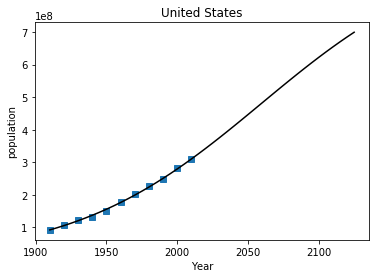
\includegraphics[width=90mm]{images/lr-graph.png}
%\caption{Results of using least squares on logistic growth \label{overflow}}
%\end{figure}

\section{Modified Lotka-Volterra}

One theorized way to model population growth is in terms of economic growth of the human population, which can be seen as being equivalent to GDP. As GDP grows, the human population naturally grows with it due to an increase in the amount of output produced by the whole population. An interesting way to model this dynamic is through a modified version of the classic Lotka-Volterra model, which simulates the interaction between predators and prey. The population can be seen as the predator with GDP as the prey since the human population is theorized to grow with GDP up to a certain point, where it slightly decreases and reaches an equilibrium. However, there are numerous theories as to how GDP and population should be viewed together, so it is more appropriate to view the model in a more general sense. 

\subsection{Transforming Lotka-Volterra}

As discussed earlier in this course, the Lotka-Volterra model in it's most basic form is written as:

\begin{align}
\begin{split}
\label{eq:lv1}
	\frac{dp}{dt} = ap - rpg \\
	\frac{dg}{dt} = rpg - bg
\end{split}
\end{align}
where $p$ is the population of the prey, $g$ is the population of the predators, and $\frac{dp}{dt}$ and $\frac{dg}{dt}$ are their annual population changes. $rpg$ describes the interaction between the two species with $r$ being a regulating coefficient, $a$ being the growth rate of the prey in the absence of predators, and $b$ being the death rate of the predators in the absence of prey. 

In order to account for other causes of variation that are not in the predator-prey system, the model can be modified to include a function $f(p, g, t)$. This can be seen as a function that modulates the growth of the prey in relation to a theoretical maximum capacity (i.e. due to the lack of natural resources). Equation \ref{eq:lv1} can now be rewritten as:

\begin{align}
\begin{split}
\label{eq:lv3}
	\frac{dp}{dt} = (\alpha_1 + \alpha_3 f)p + \alpha_2 g p \\
	\frac{dg}{dt} = \beta_1 g + \beta_2 p g
\end{split}
\end{align}
where $a, b, r$ have been replaced by $\alpha_1, \alpha_2, \beta_1, \beta_2$, which now also contain the signs. $\alpha_3f$ modulates the growth rate $\alpha_1$ in response to changes in natural resources.

From here, the model can finally be adapted to the population growth problem. $p$ can be defined as the population and $g$ as the GDP at time $t$. Putting the model into context, the function $f$ can now be determined to finally derive an appropriate model from this problem.

The most logical choice for $f$ should be an equation that reflects changing technology that improves the human population's lifestyle. This is often cited by economists as being related to GDP per capita, or $\frac{g}{p}$. $f$ can then be set as $k_1 \frac{g}{p}$ where $k_1$ is some constant that regulates the effects of GDP per capita. Using that in equation \ref{eq:lv3} yields:

\begin{align}
\begin{split}
\label{eq:lvfin}
	\frac{dp}{dt} = \alpha_1 p + \alpha_3 k_1 g + \alpha_2 g p \\
	\frac{dg}{dt} = \beta_1 g + \beta_2 p g
\end{split}
\end{align}

It is appropriate to now put the coefficients into context for a better understanding of how the model functions. $\alpha_1$ is the growth rate of the population in the absence of other factors, in terms of percentage. Similarly, $\beta_1$ is the growth rate of GDP in the absence of other factors. $\alpha_2$ and $\beta_2$ describe the interaction between population and GDP and should be negative. $\alpha_2$ is in terms of $\frac{1}{US\$}$ and $\beta_2$ is in terms of $\frac{1}{Hab.}$. $\alpha_3 k_1$ describes the positive affect that GDP has on the human population and is in terms of $\frac{Hab.}{US\$}$. In other words, it describes how many more people are born for each additional dollar that is added to the GDP. 

\subsection{Initial Simulation}

The model's authors derived what they found to be appropriate values for the parameters above when adapting the model to a global scale. The values used are: $T_0 = 1850$, $T_f = 2100$, step size $D_T = 1.0$, $P_0 = 1.15$ billion inhabitants, $G_0 = 0.21$ trillion US\$, $\alpha_1 = 0.3\%$, $\alpha_2 = \frac{-55}{10^{18} US\$}$, $\alpha_3 k_1 = 5.2 \frac{Hab.}{US \$}$, $\beta_1 = 3.1\%$, and $\beta_2 = \frac{-2}{10^{22} Hab.}$. 

These numbers, however, do not make much sense. Simple observation based on the dataset reveals that these parameters result in a massive population increase after the first iteration. The primary culprit, it seems, is their value for $\alpha_3 k_1$. As noted earlier, this value indicates how many additional people are added to the population for every dollar added to GDP. Their value indicates that there are an additional 5.2 people for every dollar, which logically does not make much sense. Potential corrections are noted below, based on additional analysis and simulations.

\subsection{Fixing World Simulation}

Additional simulations were performed both for the world and for various countries. The data was obtained from the UN World Bank dating back to 1960 and the parameters were optimized using both least squares and via minimizing a modified L2 norm score function.

Since the paper already performed simulations for the world based on a similar dataset, the result was expected to be fairly similar. However, as indicated earlier, their parameters do not make sense and were likely incorrectly reported. The resulting model indicates a substantially growing population, well past what one could reasonably expect. In order to determine the correct values, both the least squares and scoring minimization methods were used. The least squaring method, unfortunately, resulted in nonsensical results. Therefore, the scoring minimization method was utilized and produced more reasonable results. The parameters were $\alpha_1 =0.00327\%$, $\alpha_3 k_1 = \frac{4.93}{10^6} \frac{Hab.}{US \$}$, $\alpha_2 = \frac{-1.15}{10^{16} US \$}$, $\beta_1 = 7.62\%$, and $\beta_2 = \frac{-3.29}{10^{22} Hab.}$ 

The resulting graph, while matching the dataset quite nicely, does not make much logical sense. It indicates a very rapid population growth far past 10 billion people before leveling off. This is likely due to the smaller dataset being used - the paper had data going back to 1850 whereas the data used in the simulation only dates back to 1960 due to the lack of accurate population and GDP information dating back much further. However, a big takeaway from this simulation is the similarity of the parameters to the paper's. While the values were clearly different, they were fairly similar and, most notably, $\alpha_3 k_1$ was off by a magnitude of about $10^{-6}$. Based off of this, the original parameters were slightly adjusted to see if a more accurate picture could be obtained. The resulting graph is remarkably similar to what the report indicates. 

As the authors note, the model follows a logistic growth curve initially, as is expected for initial population growth. At a certain point though, the population actually begins to decrease, a significant divergence from the logistic growth model. This can be seen as a result of slowing technological growth and families becoming smaller as they become more financially stable. The population eventually levels out at an equilibrium just below 10 billion people. Meanwhile, GDP steadily grows at a sustained rate of about 1.5\%. GDP per capita is constantly rising throughout this period as technology also continues to improve. The authors point out, however, that a number of factors can have significant impacts on this model. In particular, major economic crises or significant technological achievement can raise or lower the equilibrium population. 

\subsection{United States Simulation}

In order to see how well this model adapts to other situations, additional simulations were performed at the country level. Due to the level of accuracy obtained, the least squares method was used. The first simulation was on the United States. The resulting parameters are $\alpha_1 = 1.07\%$, $\alpha_3 k_1 = \frac{2.76}{10^{7}}\frac{Hab.}{US \$}$, $\alpha_2 = \frac{-1.04}{10^{15} US\$}$, $\beta_1 = 17.9\%$, and $\beta_2 = \frac{-4.63}{10^{10} Hab.}$ 

The population is predicted to continue rising steadily until it reaches its peak at just under 375 million people in 2060 before decreasing. Unlike the model for the world population though, this decrease does not appear to level off at an equilibrium. This does not make much logical sense since there is no reasonable explanation for the population to steadily decrease that much based on GDP alone. It is likely that the model would perform far better with additional historical data. The paper's simulation of the world population used data reaching back to 1850 whereas the simulation here only used data dating to 1960 due to the lack of credible sources. Being less than a century ago, this is relatively recent and likely deprives the model of crucial information to successfully simulate this system. If additional data were used, the model would likely be similar to what was found with the world population, where an equilibrium value was attained.

One point of particular interest is the value for $\beta_1$, which indicates the growth rate of GDP in the absence of other factors. $17.9\%$ is remarkably high, especially when compared to the world as a whole. This is somewhat expected considering how developed the United States is. 

\subsection{South Africa Simulation}

The second country simulation was performed with South Africa. This is a good candidate for analysis due to its massive difference to the United States - it was only recently developed and, based off of the data, it has experienced extreme economic hardship in the past several years. Previous simulations ran on data that had a constantly increasing GDP, so this example is used to see how the model performs under more extreme conditions.

The output parameters are $\alpha_1 = 2.22\%$, $\alpha_3 k_1 = \frac{2.77}{10^{6}}\frac{Hab.}{US \$}$, $\alpha_2 = \frac{-8.31}{10^{14} US\$}$, $\beta_1 = 29.0\%$, and $\beta_2 = \frac{-5.21}{10^{9} Hab.}$. The resulting graph for population exhibits a shape similar to that seen with the world simulation, with the population rising, before eventually falling slightly and reaching an equilibrium. GDP is constantly exponentially increasing.

Despite the similarities to the world simulation, the model performed extremely poorly. While it initially follows the data quite nicely, it significantly diverges and keeps maximum population far below what the current population is. Meanwhile, GDP is shown to grow exponentially to unfathomable values that exceed even what was predicted for the world.

As mentioned earlier, the South African economy experienced hardship in recent years, unlike the other two population samples used previously. This is likely the culprit for the bizarre output and indicates that the model performs poorly for populations that do not experience economic stability and suggests that there are other significant factors that the model does not take into account.

\section{Conclusion}

As seen above, each model has its own degree of success. While the modified Lotka-Volterra model performed remarkably well in modeling the world population, it completely falls apart when analyzing a less stable source of economic and population growth, such as South Africa. Even for a well established country such as the United States, the model does not make much logical sense, despite fitting to the data quite well. 

The logistic growth model, despite its limitations, consistently produces results that make sense while also fitting the data excellently. These results suggest that the modified Lotka-Volterra model is flawed when working on smaller systems, where other factors have a much large impact on population and economic growth. It seems to assume that an economy should always be growing and fails to account for any variances in that respect. More than that, the model requires a large amount of data to function correctly, something that is unfortunately not readily available in most cases. With more data, this model would likely produce better results for the United States and similar countries. However, the model thrives on a larger scale, where fewer factors have a significant effect in population growth.

\newpage

\begin{appendices}

\section{Logistic Growth}

\begin{lstlisting}[language=Python]
def log_growth(data, times):
    # Compute dP/dt values
    dN = (data[2:]-data[:-2])/(times[2:]-times[:-2])
    P = dN / data[1:-1]
    
    X = np.asarray([np.ones(times.size - 2), data[1:-1]]).transpose()
    Y = np.asarray(P)
    alpha = np.linalg.lstsq(X,Y)[0]
    gamma = alpha[0]
    K = (-gamma) / alpha[1]
   
    # Computes from first data year to 2100
    t_estimate = np.arange(times[0], 2100, 1)
    N0=data[0]
    t_model=t_estimate-times[0]
    return K*(N0/K)*np.exp(gamma*t_model)/(1+(N0/
    K)*(np.exp(gamma*t_model)-1))
\end{lstlisting}

\section{Modified Lotka-Volterra}

\begin{lstlisting}[language=Python]
def model(t, data, params):   
    a1, a3k1, a2, b1, b2 = params
    
    x0 = [data[0][0], data[1][0]]
    
    def dpdt(x, t):
        return (a1*x[0] + a3k1*x[1] + a2*x[0]*x[1])
    def dgdt(x, t):
        return b1*x[1] + b2*x[0]*x[1]
    def dxdt(x, t):
        return np.array([dpdt(x, t),  dgdt(x, t)])
    
    # Transpose to get population and GDP in separate arrays
    return integrate.odeint(dxdt, x0, t).T 

def score(params, t, data):
    model_data = model(t, data, params)
    
    # Modified L2 norm
    return np.sum((model_data[0] - data[0])**2 + (model_data[1] - data[1])**2) 
\end{lstlisting}

\end{appendices}

\newpage

\nocite{*}
\bibliographystyle{abbrv}
\bibliography{paper}

\end{document}